\documentclass[tikz=true]{standalone}
\usepackage{graphicx, standalone}
\usepackage[compat=1.1.0]{tikz-feynman}
\usepackage{tikz}
\usepackage{amsmath, amssymb}
\usepackage{euler}
\usepackage{fontspec}
\setmainfont{MinionPro}

\renewcommand{\k}{\ensuremath\text{k}}

\begin{document}

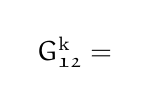
\begin{tikzpicture}[baseline=(current bounding box.center)]
    \node {$G_{\mathfrak{12}}^{\k}=$};
\end{tikzpicture}
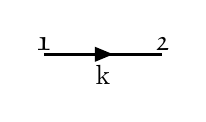
\begin{tikzpicture}[baseline=(current bounding box.base)]
	\begin{feynman}
    		\vertex (a);
    		\vertex[right=of a] (b);
    		
    		\node[above=-0.2em of a] {$\mathfrak{1}$};
		\node[above=-0.2em of b] {$\mathfrak{2}$};
		
		\diagram* {
			(a) -- [fermion, very thick, edge label'=$\k$] (b)
		};
	\end{feynman}
\end{tikzpicture}
\begin{tikzpicture}[baseline=(current bounding box.center)]
    \node {$=$};
\end{tikzpicture}
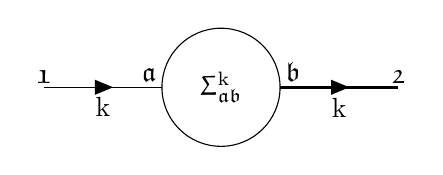
\begin{tikzpicture}[baseline=(current bounding box.base)]
	\begin{feynman}
    		\vertex (a);
    		\vertex [right=of a] (b);
    		\vertex [right=of b] (c);
    		\vertex [right=of c] (d);
    		
		\node[above=-0.2em of a] {$\mathfrak{1}$};
		\node[above left=-0.2em of b] {$\mathfrak{a}$};
		\node[above right=-0.2em of c] {$\mathfrak{b}$};
		\node[above=-0.2em of d] {$\mathfrak{2}$};    		
    		
    		\node (content) at ($(b)!0.5!(c)$) {$\Sigma_{\mathfrak{ab}}^{\k}$};
		
    		\diagram*{
        		(a) -- [fermion, edge label'=$\k$] (b),
        		(c) -- [fermion, very thick, edge label'=$\k$] (d),
    		};
   		 
    		\path (b)--++(0:0.75) coordinate (A);
    		\draw (A) circle(0.75);
	\end{feynman}
\end{tikzpicture}


\end{document}